\documentclass[]{article}
%\documentclass[]{article}

% Language-specific settings
\usepackage[english]{babel}
% Use of UTF-8 for input
\usepackage[utf8]{inputenc}
\usepackage[T1]{fontenc}
\usepackage{textcomp}

% Color
\usepackage{xcolor}

% Hyperlinks for internal references
\usepackage{hyperref}
% Change link colors and set up
\hypersetup{
	colorlinks,
    	linkcolor={red!50!black},
    	citecolor={black},
    	linktoc=all,
    	urlcolor={blue!80!black}
}

% Graphics and images
\usepackage{graphicx}
\usepackage{float}
% Tables
\usepackage{tabu}
% Subfigures
\usepackage{subfig}

\usepackage{enumerate}

% Math symbols
\usepackage{amsmath}
\usepackage{amssymb}
\usepackage{mathtools}
% Proof system
\usepackage{amsthm}

% Margin
\usepackage[margin=1.5in]{geometry}

%Bibliography
\usepackage[backend=biber, style=numeric-comp]{biblatex}
\bibliography{bibliography}
% Quotes
\usepackage{csquotes}


\setlength{\parindent}{0pt}


\title{Master-Praktikum IoT (Internet of Things)\\Written Report}
\author{Corbinian Stiglmair \& Matthias Hermann}

\pagestyle{plain}

%--------------------------------------Start------------------------------------
\begin{document}
% Titlepage + table of contents
\pagenumbering{gobble}
\maketitle
\newpage
\tableofcontents
\newpage

\pagenumbering{arabic}
% Begin text
\begin{sloppypar}
\section{Introduction}
This report is meant to document the progress made on our given project. This projects goal is to configure (and program) a system, that can give an accurate count of the current amount of persons in a room.
\section{Tools and System Components}
Our Prototype consists of the following components:
\begin{itemize}
	\item Breadboard\footnote{TRU COMPONENTS 0165-40-4-28010 Steckplatine}
	\item Adafruit Feather M0 Board (with RFM95 LoRa Radio - 900MHz - RadioFruit)
	\item OLED Screen\footnote{Joy-it SBC-OLED01}
	\item Photoelectric Barrier\footnote{Iduino 1485329}
	\item Jumper Cables
	\item USB Cable
\end{itemize}
\section{Approach}
Instead of focusing on the individual work sessions, this report will instead describe how partial subgoals were achieved and how the subgoals are intertwined with each other.
\subsection{Adafruit Feather M0 Board}
In order to compile code for this board the installation of the Boards \textit{Arduino SAMD Boards} and \textit{Adafruit SAMD Boards} is required.
\subsection{OLED-Screen}
the OLED-Screen requires the installation of the two libraries \textit{Adafruit SSD 1306} and its dependency \textit{Adafruit GFX Library}.
\subsection{Photoelectric Barrier}
The barrier activates, whenever something obstructs its two endpoints. See, for reference \eqref{img:iduino_highlighted}.\\
\begin{figure}
	\centering
	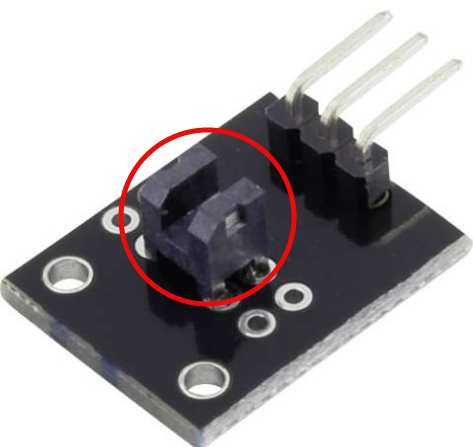
\includegraphics[width=0.5\textwidth, keepaspectratio]{./images/iduino_highlighted.png}
	\caption{The photoelectric sensor (Iduino 1485329) with the corresponding endpoints highlighted.}\label{img:iduino_highlighted}
\end{figure}	
We use this to simulate the entries of persons by passing a black stripe through each of the two sensors.
\subsection{Interrupt Handling}
We attach interrupt routines to both our sensors\footnote{as described here \url{https://www.arduino.cc/reference/de/language/functions/external-interrupts/attachinterrupt/}}. One advantage of this is, that the CPU can enter a power-save mode.
\newpage
% Sources
\printbibliography

\end{sloppypar}

\end{document}
